% Slides for 2025-04-29
% To create a slide, use the following:
% \begin{frame}{TITLE}
%     BODY
% \end{frame}

% To create a slide with a bullet list, use the following:
% \begin{frame}{TITLE}
%     \begin{itemize}
%         \item ITEM 1
%         \item ITEM 2
%     \end{itemize}    
% \end{frame}

% To create a slide with numbered list, use the following:
% \begin{frame}{TITLE}
%     \begin{enumerate}
%         \item ITEM 1
%         \item ITEM 2
%     \end{enumerate}
% \end{frame}

% To create a slide with a graphic:
% 1. Add the graphic to this folder (named picture.png)
% 2. Use the following:
% \begin{frame}{TITLE}
%     \centering
%     \includegraphics[height=0.7\textheight,width=0.7\textwidth,keepaspectratio]{picture.png}
% \end{frame}

% To create a slide with two columns, use the following:
% \begin{frame}{TITLE}
%     \begin{columns}
%         \begin{column}{0.5\textwidth}
%             COLUMN 1 BODY
%         \end{column}
%         \begin{column}{0.5\textwidth}
%             COLUMN 2 BODY
%         \end{column}
%     \end{columns}
% \end{frame}

\begin{frame}{Rust Pipeline}
  \begin{columns}[c]
      \column{0.48\textwidth}
        \centering
        \textbf{Tail Correct}\\[1ex]
        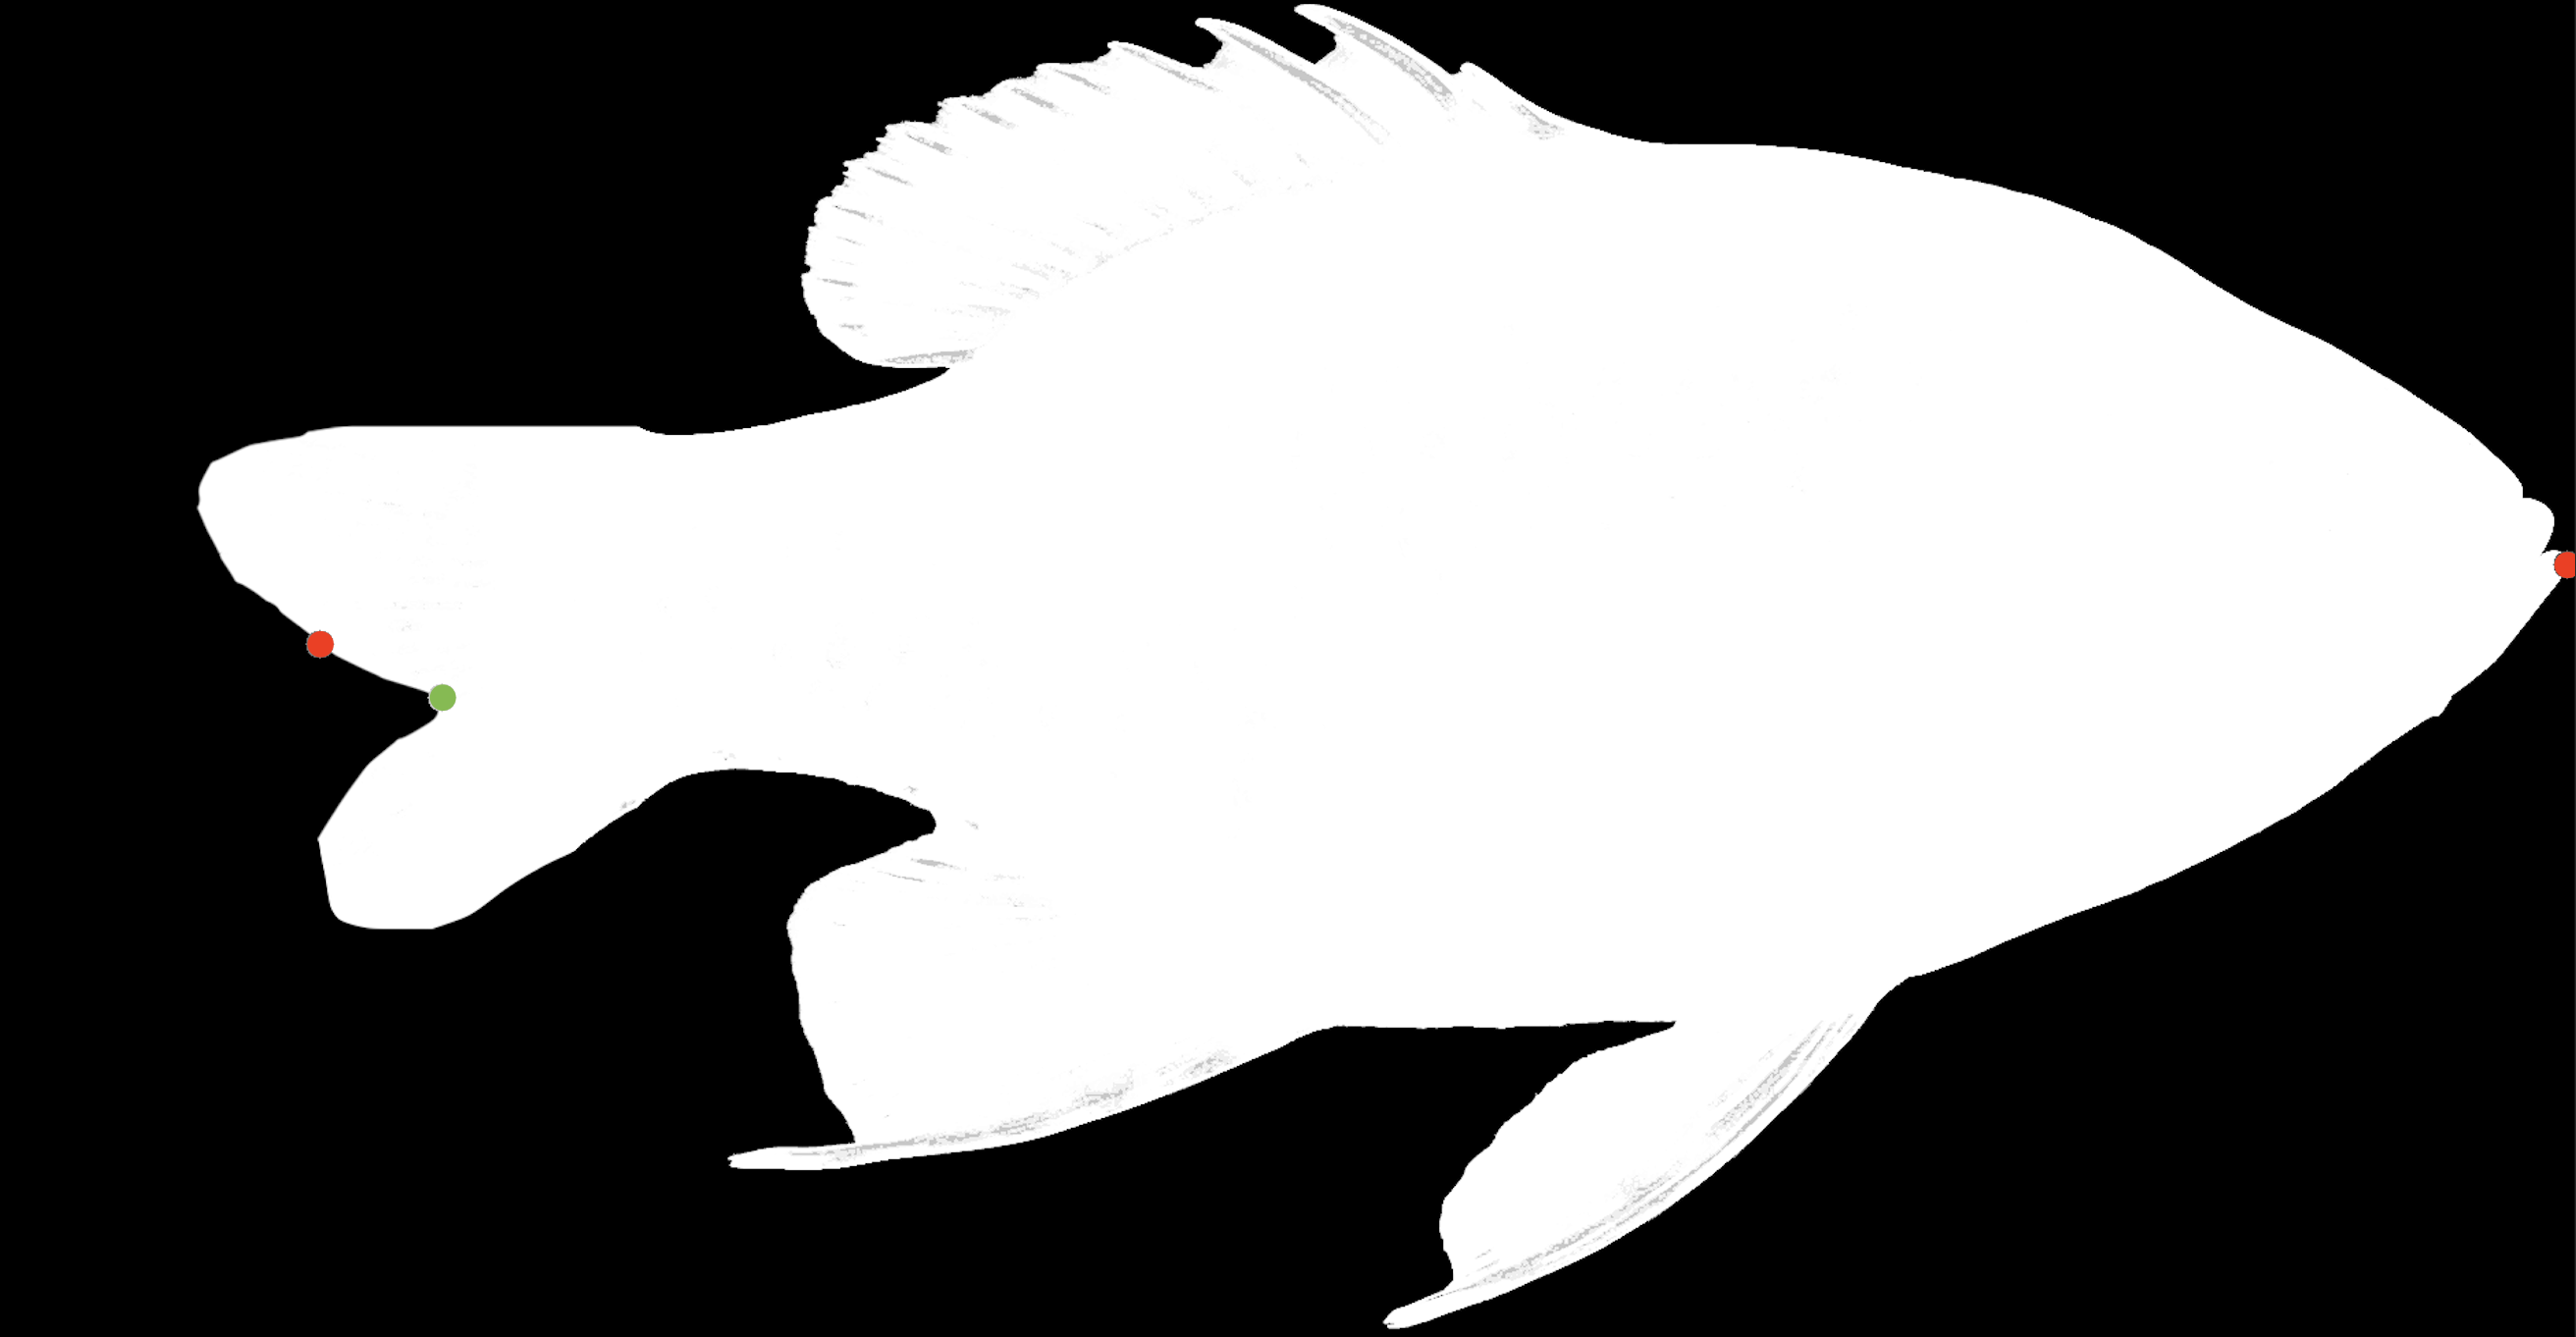
\includegraphics[height=0.48\textheight,keepaspectratio]{./images/fish2_out.png}
  
      \column{0.48\textwidth}
        \centering
        \textbf{Tail/Head Distinction}\\[1ex]
        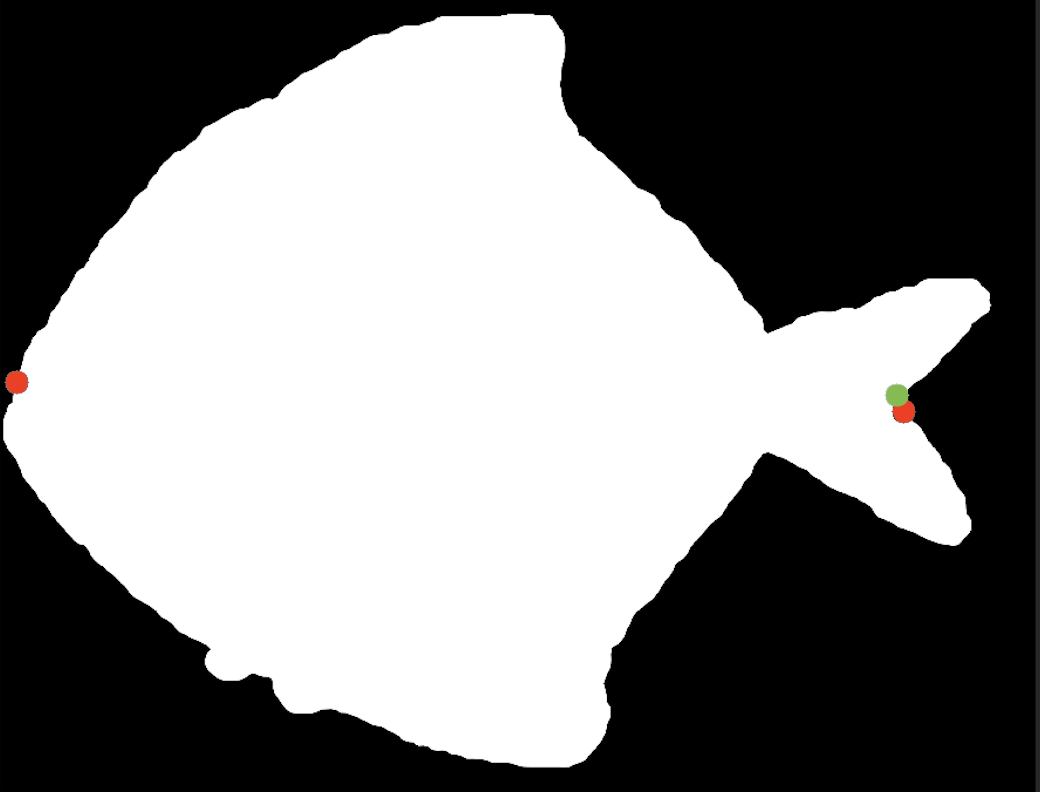
\includegraphics[height=0.48\textheight,keepaspectratio]{./images/fish6_out.png}
  \end{columns}
      \begin{enumerate}
        \item Head correction
        \item Test different radius thresholds
        \item Compare distinction with old python pipeline
    \end{enumerate}
\end{frame}

\begin{frame}{Underwater Renderer}
    \begin{enumerate}
	    \item Done: Testing FP32 and 64. Expects around 200 in 1 million calculations to have more than 0.1 percent error, and 10 to have more than 1 percent
			\item Re-evaluate Platforms: FP64 suffers very heavy performance penalty on all consumer GPUs, still heavy penalty on NVIDIA server GPUs
			\item Consideration for building program for MI210 as no FP64 penalty, and by extension switching to ROCm/HIP
    \end{enumerate}
\end{frame}
